\chapter{Analýza}

\section{Monitorovanie vibrácií a šoku}
Vibrácie sú periodickým kmitaním hmoty okolo rovnovážnej polohy vznikajúce excitáciou látky, ktorej je dodaná potenciálna energia, a zo 
zákona zachovania energie je následne premieňaná na kinetickú energiu. V realite dochádza pôsobením trenia k útlmu voľného oscilačného 
pohybu s časom  a pohybová energia sa uvoľňuje v podobe tepelnej alebo akustickej emisie do okolitého prostredia. Častejšie ako presné 
harmonické kmity sú pozorované náhodné vibrácie, ktorých vývoj nevieme dopredu predvídať. Naproti tomu šok, alebo aj prechodový jav, je 
náhle uvoľnenie kinetickej energie krátkeho trvania oproti prirodzenej oscilácii systému. 

Význam a dôležitosť sledovania vibrácií spočíva v ich výskyte u každého mechanického zariadenia a je zapríčinená pohybom jednotlivých 
súčiastok a trením v ložiskách. Ich nadmerná prítomnosť býva spôsobená opotrebením dielov stroja alebo nevyvážením rotačných častí, 
zakliesňovaním ozubených kolies, ako dôsledkoch iných technických defektov. V prevažnej väčšine prípadov ide o nežiaduci jav nakoľko 
zakladá zníženiu účinnosti so zvýšením hlučnosti ako vedľajšiemu produktu. 

Ďalšou oblasťou hojnej prítomnosti vibrácií je preprava osôb alebo tovaru cestnými a železničnými dopravnými prostriedkami, kde sú 
zapríčinené nerovnosťami povrchu vozovky alebo koľaje v bode styku s kolesami vozidla. Na zvýšenie ovládateľnosti vozidla a komfortu 
pasažierov sú kabíny odpružené od kolies tlmičmi. Lietadlá sú zasa pod vplyvom trenia vzduchu s trupom a krídlami konštrukcie, ktoré je 
ďalej zosilnené vzdušnými prúdmi a turbulenciami. 

Druhým významným faktorom podieľajúci sa na tvorbe vibrácii je aparát, ktorý uvádza vozidlo do pohybu alebo zastavuje, čiže hnací 
najčastejšie spaľovací, dieselový alebo elektrický motor a brzdový systém. Jedná sa najmä o vplyv pohybu piestov, alebo rotora u 
elektrických vozidiel, a prenosu otáčavého pohybu motora cez oje hriadeľa na nápravy. ABS brzdový systém prítomný pri väčšine
automobilov zabraňujú šmyku striedavým zomknutím a uvoľňovaním brzdových kotúčov, čo má tiež vplyv na podmienky počas jazdy.

Detekciou nežiaducich vibrácií v preprave sa dokáže zabezpečiť aj bezpečnosť pasažierov včasnou výmenou súčiastky, ktorá by ovplyvnila 
prevádzkyschopnosť v kritických momentoch. Ich eliminácia dokáže predísť nenávratnému poškodeniu krehkých materiálov alebo 
znehodnoteniu reaktívnych substancií, či dokonca ich aktivácii v prípade výbušnín a pyrotechniky.

V neposlednom rade sú vibrácie súčasťou potenciálne nebezpečných prírodných úkazov a ich správna identifikácia má za následok varovania 
pre preventívnu evakuáciu obyvateľstva v oblasti, ktoré bude zasiahnutá zemetrasením, či erupciou sopky vedúcimi k ohrozenia zdravia 
osôb a poškodenia majetku.
 
\subsection{Meranie fyzikálnej veličiny akcelerácie}
Pohyb mechanického systému vystaveného vonkajším silám sa nazýva odozva, ktorej správanie opisuje zjednodušený model s jedným stupňom 
voľnosti (1DOF) kmitajúceho telesa s pružinou a tlmičom \cite{vibrations-shock}. 

\begin{figure}[h]
	\centering
	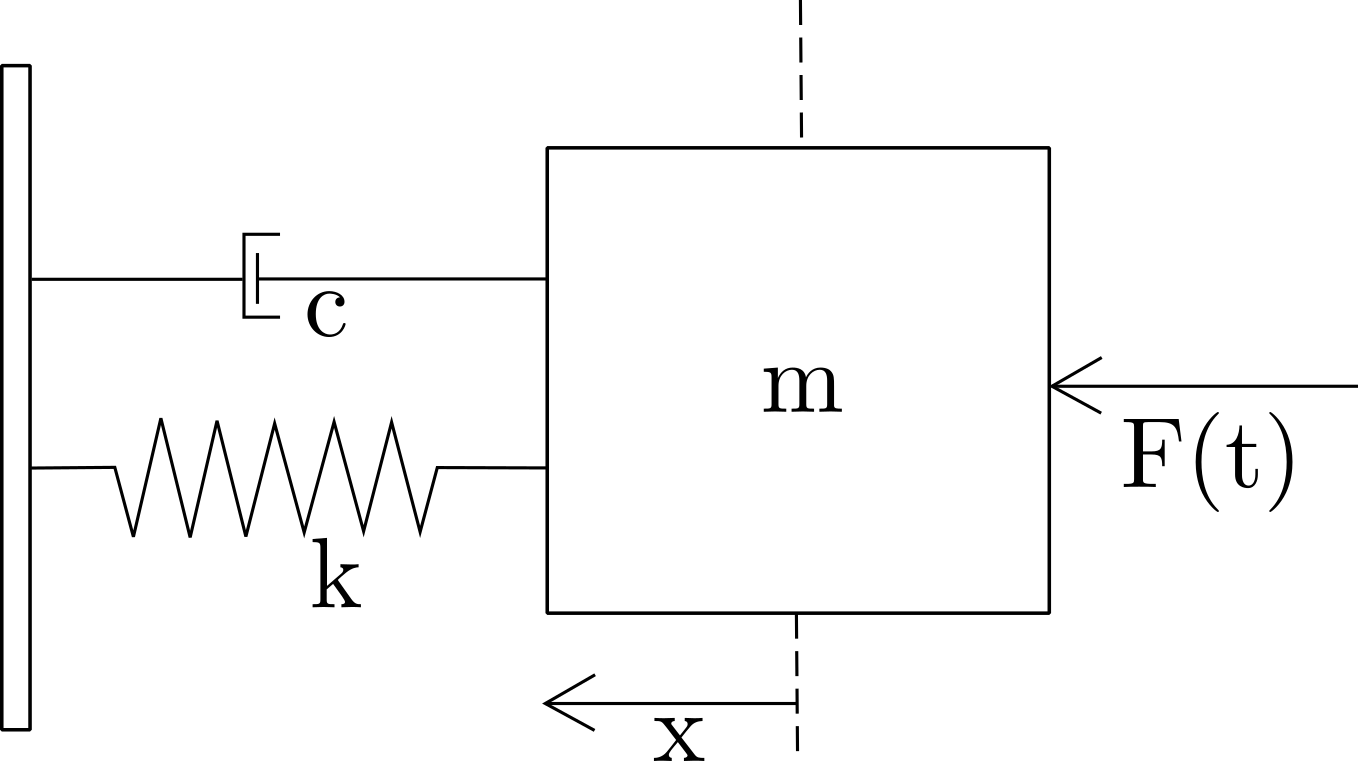
\includegraphics[width=0.7\textwidth]{figures/mass-spring-damper-model.png}
	\caption{Model oscilujúceho systému s pružinou a tlmičom}
\end{figure}

Pri pôsobení vonkajšej sily $F$ na hmotu upevnenú na pružine vznikajú nútené vibrácie, ktoré ju vychyľujú z rovnovážnej polohy. Uvedená sila je charakterizovaná druhým Newtonovým zákonom v tvare $F = ma$, kde $m$ je hmotnosť telesa a $a$ predstavuje zrýchlenie. V protismere pôsobí sila vyvolaná pružinou $F_s = -kx$ a tlmiacim členom $F_d = -cv$, kde $k$ je tuhosť pružiny ovplynená jej konštrukciou, $c$ je tlmiaci koeficient, $x$ je vychýlenie z rovnovážneho stavu, a $v$ rýchlosť vychýlenia. Fyzickým obmedzením  telesa, ktorým je viazaný na pevnú podložku dochádza pri zanedbaní deformácie k takmer zaručenému návratu do rovnovážnej polohy a to nám umožňuje merať intenzitu vibrácií cez zrýchlenie ťažidla. Sčítanie zložiek síl podieľajúcich sa na dynamike telesa vyúsťujú v obyčajnú diferenciálnu rovnicu na výpočet výslednej sily v jednom smere.
\begin{ceqn}\begin{align}
 	F(t) = ma - cv - kx
\end{align}\end{ceqn}
Pri použití trojosového akcelerometra, kedy sú evidované všetky tri priestorové súradnice časovo-premennej akcelerácie dostávame 
nasledujúcu rovnicu vo vektorovom tvare: 
\begin{ceqn}\begin{align}
   \vec{a}(t) = \frac{\vec{F}(t)}{m}
\end{align}\end{ceqn}
Magnitúda akcelerácie s troma súradnicami je daná $L_2$ normou vektora $\vec{a} = (a_x, a_y, a_z)$:
\begin{ceqn}\begin{align}
   |a| = \sqrt{a_x^2 + a_y^2 + a_z^2}
\end{align}\end{ceqn}

\subsubsection{MEMS kapacitný akcelerometer}
Bežné inerciálne senzory na meranie zrýchlenia priamočiareho, ale aj rotačného pohybu (gyroskop), sa vyrábajú technológiou 
\emph{MEMS – mikromechanický systém}, kedy je celé zariadenie vrátane všetkých mechanických súčastí umiestnené na kremík procesom 
mikrovýroby vo viacerých vrstvách. Sila spôsobujúca zrýchlenie je potom meraná vychýlením vstavanej odpruženej hmoty vzhľadom 
na pevné elektródy, ktoré môžu byť usporiadané jednostranne alebo ako diferenčný pár \cite{mdof-mems-accelerometers}.

\begin{figure}[h]
	\centering
	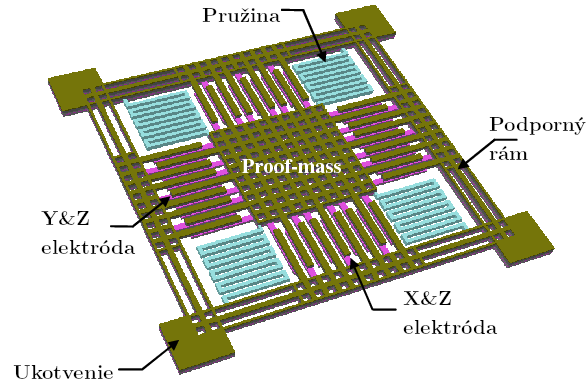
\includegraphics[width=0.8\textwidth]{figures/mems-accelerometer.png}
	\caption{Mikroštruktúra 3DOF MEMS kapacitného akcelerometra}
\end{figure}

Pri diferenčnom páre spôsobí pohyb doštičky ťažidla medzi elektródami zmenu kapacít a ich rozdielom je možné zistiť aplikovanú silu a 
cez uvedený vzťah zrýchlenie. Na zvýšenie celkovej kapacity sa používa viacero párov elektród zapojených paralelne. Pred prevodom na 
číslicový signál musí napäťová úroveň zo senzora prejsť úpravou zahŕňajúcou nábojovocitlivý predzosilňovač, osovú demoduláciu a anti-
aliasingové filtrovanie. Viacosové akcelerometre vyžadujú viaceré opísané štruktúry orientované kolmo na seba podľa počtu vyžadovaných 
stupňov voľnosti, pričom v skutočných senzoroch vždy existuje aspoň minimálna závislosť medzi osami rádovo najviac v jednotkách 
percent. Teplota ovplyvňuje citlivosť MEMS akcelerometrov len nepatrne v stotinách percenta na stupeň Celzia.

Akcelerometre sa odlišujú v niekoľkých dôležitých vlastnostiach, ktoré zvyknú byť nastaviteľné vo výrobcom stanovenom rozsahu 
prípustných hodnôt s príslušnými toleranciami \cite{accelerometer-mechanics}. 
\emph{Citlivosť} stanovuje najmenšiu rozlíšiteľnú zmenu v odčítanom napätí ku zmene externého pohybu respektíve zrýchlenia.
Uvádza sa v jednotkách \emph{mV/g} (milivolt na tiažové zrýchlenie) pri analógovom výstupe, alebo \emph{mg/LSB} (mili-g 
na najmenej významový bit). pri senzoroch so vstavaným analógovo-digitálnym prevodníkom. Jednotka \emph{mg/LSB} vyjadruje 
o koľko sa zmení zrýchlenie keď zvýšime alebo ponížime binárne číslo na výstupe o jedna. Niekedy sa namiesto 
citlivosti uvádza mierka pre presnosť ako prevrátená hodnota citlivosti v \emph{LSB/g}. Tiažové zrýchlenie $g$ sa mierne líši podľa 
zemepisnej šírke, ale stanovený prepočet na jednotky SI je $1 g = 9.80665\,m/s^2$ 
\footnote{\url{https://physics.nist.gov/cgi-bin/cuu/Value?gn|search_for=acceleration}}. 

\emph{Dynamický rozsah} sa uvádza v tiažovom  zrýchlení $g$. Hovorí o najmenšej a najväčšej rozlíšiteľnej hodnote zrýchlenia nad 
úrovňou ktorej už dochádza k skresleniu signálu orezaním špičiek. S nevyhnutnými drobnými nepresnosťami výroby mikromechaniky je tzv. 
\emph{zero-g napätie} popisujúce odchýlku skutočného od ideálneho výstupu, keď na sústavu nepôsobí žiadne zrýchlenie. Za ideálnych 
okolností bez pohybu na vodorovnom povrchu namerajú osi $x$ a $y$ zrýchlenie $0g$, zatiaľčo na $z$ pôsobí $1g$. Očakávaním je nulová 
hodnota výstupného napätia a tým aj výstupného registra.

\emph{Šírka pásma} senzora v $Hz$ predurčuje rozsah frekvencie vibrácií, ktoré je možné zachytiť. Podmienená je zvolenou početnosťou 
čítania akcelerácie za sekundu, čiže vzorkovacou frekvenciou. Stanovuje sa tiež nastaviteľným parameterom \emph{ODR} (Output Data Rate) 
- výstupný dátový tok, pričom šírka pásma je spravidla polovicou ODR. Menej uvádzanou vlastnosťou býva \emph{frekvenčná odozva} 
senzora, ktorá určuje o koľko sa v rámci tolerancie odlišuje skutočná citlivosť od referenčnej pre zodpovedajúcu frekvenciu vibrácii.
Na meranie zrýchlenia má nevyhnutný vplyv šum zapríčinený Brownovým pohybom a nedokonalosťou skutočných materiálov v štruktúre
akcelerometra. Intenzita šumu rastie inverznou odmocninou so šírkou pásma, čiže s častejším meraním získavame menšiu presnosť. Pri dostatočnom odstupe signálu od šumu, $SNR = \frac{P_{signal}}{P_{šum}}$, umožňuje hardvér akcelerometra vzorkovať amplitúdy až
nad stanovený prah generovaním prerušenia, čím sa dokáže efektívne zbaviť nevýznamných fluktuácií.

\subsubsection{Analógovo-digitálny prevodník}
Spojitá napäťová úroveň transformuje analógovo-digitálny (A/D) prevodník pre spracovanie digitálnym systémom do množiny diskrétnych 
hodnôt. Vstupný signál najprv prechádza fázou vzorkovania, kedy sa vzorky zaznamenávajú v pravidelných intervaloch. Počet vzoriek 
odčítaných za sekundu je vyjadrený vzorkovacou frekvenciou $f_s$ v $Hz$. Časový rozdiel medzi vzorkami, nazývaný perióda vzorkovania, 
je prevrátenou hodnotou vzorkovacej frekvencie $T_s = \frac{1}{f_s}$. Pre presnú rekonštrukciu pásmovo obmedzeného signálu v hraniciach 
$[-f_{max}; f_{max}]$ je nevyhnuté podľa Nyquist-Shannonovej vety o vzorkovaní, aby vzorkovacia frekvencia bola najmenej dvojnásobkom 
maximálnej frekvencie snímaného signálu.
\begin{ceqn}\begin{align}
   f_s \geq 2 \cdot f_{max} 
\end{align}\end{ceqn} 

Každej vzorke je následne v procese kvantovania priradená diskrétna hodnota s konečným počtom $n$ bitov, ktorá je najbližšia možná ku 
skutočnej hladine analógového vstupu. Dochádza pritom k istému zaokrúhľovaniu z dôvodu nepresnosti vyjadrenia spojitej domény amplitúd 
diskrétnym číslom. Tento jav označujeme ako kvantizačný šum, ktorý je najviac polovicou z maximálnej rozlíšiteľnej zmeny signálu a 
trpia nim všetky existujúce A/D prevodníky. Rovnako tak sa u všetkých prevodníkov prejavuje aspoň nepatrná miera nelinearity výstupného 
kódu, chýbajúce kódy alebo ich nemonotónnosť.

\begin{figure}[h]
	\centering
	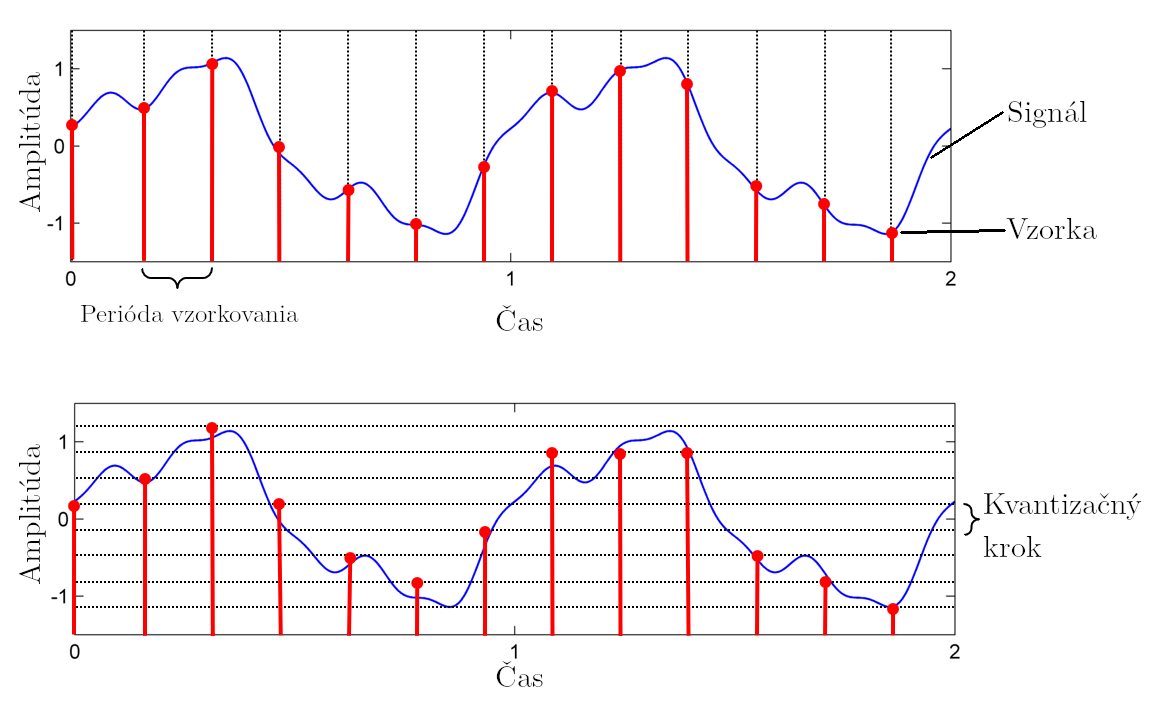
\includegraphics[width=0.8\textwidth]{figures/analog-to-digital-conversion.png}
	\caption{Digitalizácia signálu v analógovo-digitálnom prevodníku}
\end{figure}

Prevodníky integrované priamo s inerciálnymi jednotkami sa vyhotovujú v rozlíšeniach 12, 16 alebo 20 bitov. Umožňujú tak pripojiť akcelerometer rovno na sérové zbernice \emph{SPI} alebo \emph{I2C}. Všeobecne platí, že pri $n$ bitoch je k dispozícii $2^n$ rozličných čísel. Kódovaním v dvojkovom doplnku pre zachytenie záporných hodnôt sa uvažuje s intervalom $[-2^\frac{n}{2}; 2^\frac{n}{2} - 1]$. Napríklad pri 12-bitovom A/D prevodníku s referenčným napätím $3.3V$ je teoreticky najmenšia rozlíšiteľná zmena na najmenej významový bit $3.3V / 2^{12} = 0.81 mV$. Ak je rozhranie senzora priamo vybavené analógovým výstupom nič nebráni v použití presnejšieho prevodníka, napriek tomu najmenší merateľný dielik je zdola stále ohraničený citlivosťou akcelerometra. 

Číslicovú hodnotu v dvojkovom doplnku získanú konverziou $\hat{x}$ je z dôvodu širšej zrozumiteľnosti žiaduce prepočítať na štandardné fyzikálne jednotky pre zrýchlenie, $a$ v $m/s^2$). $R$ prestavuje nastavený dynamický rozsah v jednotkách $g$ a $n$ je počet bitov A/D prevodníka.
\begin{ceqn}\begin{align}
   a = \hat{x} \cdot \frac{R \cdot g}{2^\frac{n}{2}}
\end{align}\end{ceqn}

Ako bolo spomenuté ohľadom vlastností MEMS akcelerometrov, presnejší prevod dosiahneme zužitkovaním deklarovanej citlivosti senzora pri danom dynamickom rozsahu $S_R$ udávaného v $mg/LSB$.
\begin{ceqn}\begin{align}
   a = \hat{x} \cdot \frac{S_R \cdot g}{1000}
\end{align}\end{ceqn}

\subsubsection{Vlastnosti bežných akcelerometrov}
Na ilustráciu uvádzame parametre zvolených najrozšírenejších typov akcelerometrov. Akcelerometer LSM9DS1 \cite{lsm9ds1} umožňuje cez 
zbernicu SPI alebo I2C zvoliť zo štyroch dynamických rozsahov, pričom každé rozpätie sa vyznačuje svojou citlivosťou. Zvolením menšieho 
dynamického rozsahu zvýšime citlivosť. LSM9DS1 funguje pri rozsahoch $\pm2$g, $\pm4$g a $\pm8$g a $\pm16$g, postupne s citlivosťami 
$0.061$ mg/LSB, $0.122$ mg/LSB, $0.244$ mg/LSB, $0.732$ mg/LSB. Výstupný dátový tok (ODR) je možné nastaviť na $10$Hz, $50$Hz, 
$119$Hz, $238$Hz, $476$Hz a najvyššie na $952$ Hz. Navzorkované hodnoty sú ukladané do 16-bitového výstupného registra v 
dvojkovom doplnku. 

Nízkoenergetický 3DOF MEMS akcelerometer ADXL362 \cite{adxl362} so spotrebou $2\,\mu A$ pri $100$Hz disponuje
rozsahmi $\pm2$g, $\pm4$g a $\pm8$g s citlivosťami $1$, $2$ a $4$ mg/LSB. Dostupné vzorkovacie frekvencie 12-bitového A/D prevodníka sú $12.5 - 400$Hz v 8 krokoch vždy po násobkoch predošlého kroku. Pre rýchlejšie čítanie pri nižšom rozlíšení dokáže senzor zakódovať dáta do 8-bitového registra.

Vyrábajú sa tiež akcelerometre s väčšími dynamickými rozsahmi a nízkym šumom, ide napríklad o ADXL356 a ADXL357 \cite{adxl357} so škálami $\pm 10$g, $\pm 20$g a $\pm 40$g s citlivosťou $0,019$ mg/LSB po $0,078$ mg/LSB a rozlíšením A/D prevodníka 20 bitov pri ODR $4 - 4000$Hz. ADXL357 ponúka priamo analógové výstupy s citlivosťou $20 - 80$ mV/g pri napájaní $3.3$ V.

\subsection{Odvodzovanie rýchlosti a polohy zo zrýchlenia}
fyzikálne vzťahy pre polohu, rýchlosť a zrýchlenie, numerická derivácia a integrácia (obdĺžníkové, lichobežníkové, Simposonovo pravidlo) \cite{integration-acceleration-envelopes}

%\begin{figure}[h]
%	\centering
%	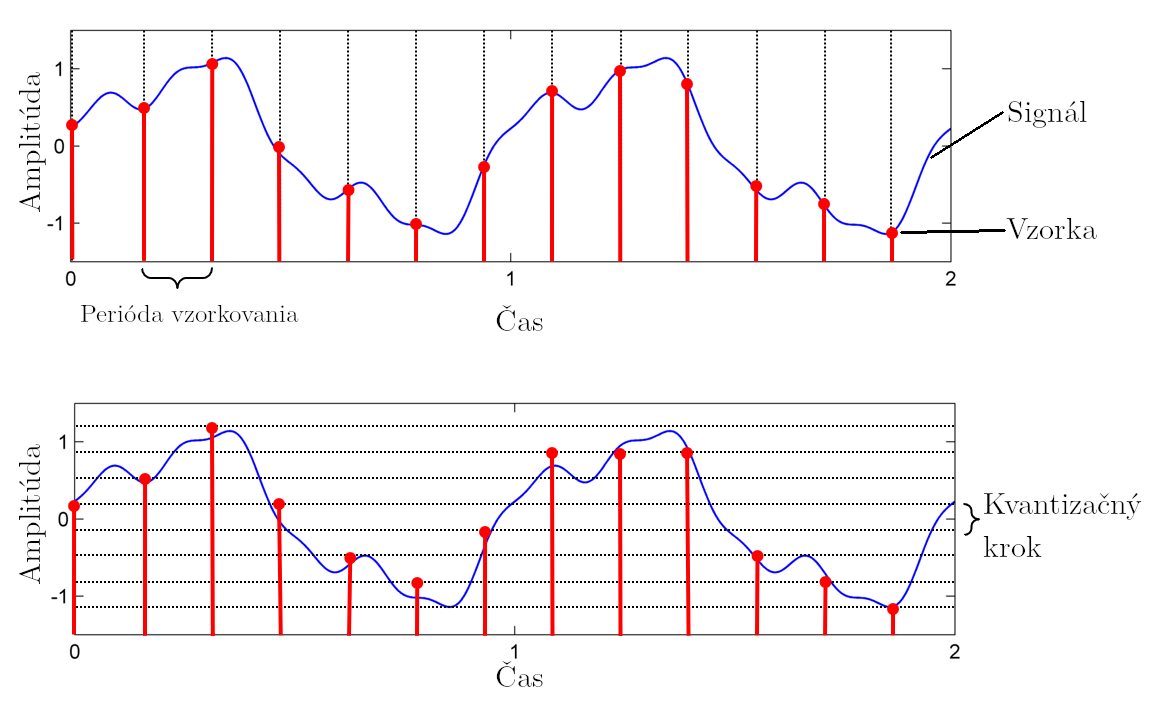
\includegraphics[width=0.8\textwidth]{figures/analog-to-digital-conversion.png}
%	\caption{Porovnanie metód numerickej integrácie}
%\end{figure}



\section{Metódy analýzy signálu v časovej doméne}
časový rad, okná
\cite{time-series-analysis} \cite{practical-time-series} \cite{generalized-esd} \cite{twitter-esd}, 
online algoritmus \cite{online-anomaly-detection}, 
požiadavky na efektívne algoritmy
	

\subsection{Číselné charakteristiky štatistického rozdelenia}
bodové odhady momentov. výberový priemer = stredná hodnota, výberový rozptyl (Welfordov online algoritmus), šikmosť, špicatosť, kvantily, normálne rozdelenie pravdepodobnosti

%\subsection{Prúdové algoritmy}
%stream algorithm models, Data Stream Model - cash register, turnstile, time series, window model
%Odhad momentov, Rátanie frekvencií, Zistenie či sa dopyt už vyskytol
%Count–min sketch (\url{https://florian.github.io/count-min-sketch/}) - probabilistická dátová štruktúra

\subsection{Algoritmy na rozpoznávanie špičiek}
lokálne minimá a maximá extrémy - cez prvú a druhú deriváciu,
topografická prominencia a izolácia - relatívna výška vrchola / extrému
vyhladzovanie: mean filter, derivative filter (diskrétny derivačný operátor) - sobel filter na , Savitzky–Golay filter
Vzájomná korelácia - jadra vrchola a signálu
detect peaks in a signal and to measure their positions, heights, widths, and/or areas

\cite{spectrometry-peak-detection}
\cite{survey-peaks-valleys}
\cite{peek-mountaineer-method}
\cite{ecg-r-peak-detection}
\cite{ampd-algorithm}

\subsubsection{Jednoduchý detektor vrcholov}
Preskočí špičky s absolútnou magnitúdou menšou ako `height`. Vo vnútornom cykle zisťuje či je bod vyššie ako všetkých `k` susedov doprava a doľava s toleranciou `epsilon`.

\begin{equation}
\forall c \in \{y_{i-k}, ... y_{i+k}\} - \{y_i\}; \; y_i - c \geq -\epsilon
\end{equation}

\begin{lstlisting}[language=Python]
def find_peaks(y: list, k: int, epsilon: float=0, height: float=None) -> list:
    spikes = []
    
    for a in range(k, y.size - k): 
        if height is not None and abs(y[a]) < height:
            continue
        locmax = True
        for b in range(-k, k):
            if b != 0 and y[a + b] - y[a] > epsilon:
                locmax = False
        if locmax:
            spikes.append(a)

    return spikes
\end{lstlisting}
\url{https://terpconnect.umd.edu/~toh/spectrum/PeakFindingandMeasurement.htm}

\subsubsection{Algoritmus Negative Zero-Crossing}
Nájdi vo n-krát vyhladenom signále body, že platí: $f'(x) = 0$, kde $f''(x) < 0$ a $|f''(x)| > \theta$. Pre odstránenie hraničných efektov použiť mód 'valid' s prísušným posunom hraníc polí.

Diskrétna verzia:
$$f'(x) = 0 \; \mathrm{(Dotyčnica)} \implies |y_{i+k} - y_{i-k}| \leq \epsilon \;\mathrm{(Sečnica)}$$
$$f''(x) < 0 \implies (y_{i+k} - y_i) - (y_i - y_{i-k}) < 0$$
$$|f''(x)| > \theta \implies |(y_{i+k} - y_i) - (y_i - y_{i-k})| > \theta$$

Parametre: 
\begin{itemize}
\item $\epsilon$: tolerancia pre nulovú deriváciu
\item $\theta$: strmosť druhej derivácie, čiže špicatosť vrchola
\item $k$: polovica dĺžka sečnice pre výpočet prvej derivácie
\item $n$: veľkosť konvolučného jadra
\item $smooth$: počet vyhladzovaní
\end{itemize}

\subsubsection{Algoritmus horského turistu}
Obsahuje pamäťový efekt pre dočasné zmeny a berie ich do úvahy ak lokálne záchvevy prekročia tolerovanú úroveň. Ak sa zmení 'slope' oproti predošlému kroku DeltaY, tak hneď neoznačí za zmenu medzi dolinou a vrcholom, ale až po prekročení nastavených prahov. Skutočnosť z reality: jama != údolie


\subsection{Online detekcia anomálií a odchýliek pozorovaní}
Outlier je pozorovanie, ktoré sa odchyluje, tak významne od ostatných pozorovaní, že vzbudzuje
podozrenie, že bolo vytvorené odlišným mechanizmom. Normálne dáta, Šum, Anomálie (slabé a silné odchýlky)
Výstupy algoritmov na detekciu výchyliek: 
\begin{itemize}
\itemsep0pt
\item Outlier skóre - miera vychýlenosti bodu
\item Binárne štítky - binárne štítky, označenie, či je bod anomália alebo nie.
\end{itemize}
Algoritmy na anomálie vytvárajú model normálnych vzorov v dátach a skóre vychýlenosti je dané deviáciou od týchto vzorov.
\cite{outlier-analysis} 
Hampel filter

\cite{survey-univariate-time-series} 
Množstvo prenášaných a spracovaných dát prevyšuje ľudskú schopnosť manuálneho prieskumu. Anomália je pozorovanie alebo postupnosť pozorovaní, ktoré sa významne odchyluje od distribúcie zvyšku dát. 
\begin{itemize}
	\item Bodové anomálie - $x_t$ je bodová anomália ak sa jeho hodnota významne odlišuje od všetkých 		
		bodov v intervale $ [x_{t-k}; x_{t+k}] $
	\item Kolektívne (disonanancie) - jednotlivé body nepredstavujú anomálne správanie, až ak vezmeme dlhšiu postupnosť môže byť označená za anomáliu.
	\item Kontextové výchylky / anomálie - body sú normálne v určitom kontexte, ale v inom anomálne.
\end{itemize}		

\cite{review-outlier-datection} \cite{anomaly-detection-algorithms}
\begin{equation}
|x - \hat{x}| \geq \theta 
\end{equation}

Bežiaci filter  
\cite{anomaly-detection-models}

\subsubsection{Metriky pre binárny klasifikátor}
Skóre anomálnosti, 	binárny klasifikátor, 
Falošne pozívny - proces je normálny, ale registrujeme neočakávané správanie, 
Falošne negatívny - proces je abnormálny, ale správanie prechádza bez povšimnutia
Matica zámen, Precision, Recall, 
ROC - kvalita binárneho klasifikátora v závislosi od prahu, AUC
\cite{wsn-outlier-detection-survey}

Z-score a Z-test: 
\begin{equation}
z = \frac{|x - \mu|}{\sigma} \approx \frac{|x - \bar{x}|}{S}
\end{equation}
Bežiaci priemerovací filter \cite{anomaly-detection-models}

Zisťovanie výchyliek testovaním štatistických hypotéz: 
generalized extreme Studentized deviate test \cite{generalized-esd} 

Median Absolute Deviate (robustná štatistika na určenie vychýlenosti od normálu)
\begin{equation}
MAD = \mathrm{median}(|X_i - \bar{X}|)
\end{equation}


\section{Frekvenčná a časovo-frekvenčná analýza signálu}
vlastnosti frekvenčného spektra, decibele, spektrogram, odstup od šumu (SNR), power spectrum density (dbFS), spektrálny analyzátor 

\subsection{Fourierová transformácia}
Diskrétna fourierová transformácia mapuje signál dĺžky $N$ do množiny $N$ diskrétnych frekvenčných komponentov. \cite{signal-processing}
\begin{equation}
X = \mathbf{W}x; W_{nk} = e^{-i\frac{2\pi}{N}nk} = W_N^{nk}
\end{equation}
Inverzná transformácia
\begin{equation}
x = \frac{1}{N}\mathbf{W}^H X
\end{equation}

Integrálne transformácie: Fourierová transformácia (CFT, DFT), Kosínusová transfomácia (MDCT), Vlnková transformácia (CWT) \cite{dct} \cite{casove-frekvencia-analyza-signalu}

\begin{equation}
T(n) = \int{f(t) K(t,x) \mathrm{dt}}
\end{equation}

\begin{equation}
\mathcal{F}: X(\omega) = \int_{-\infty}^{+\infty}{x(t) \cdot e^{-i\omega t} \mathrm{dt}}
\end{equation}

\subsection{Algoritmus FFT pre DFT a DCT}
Opis DIT radix-2 FFT algoritmus komplexných, reálny, pre MDCT \cite{fft-blackbox}

\begin{equation}
X(m) = \sum_{n = 0}^{N-1}{x(n) \cdot e^{-i2\pi n m / N}}
\end{equation}

Frekvenčné rozlíšenie
\begin{equation}
\Delta f = \frac{f_s}{N}
\end{equation}

\subsection{Oknové funkcie}
Gaborová transformácia, Prehľad okien a ich transformácií (sinc), Efekt oknových funkcií na spectral leakage, výhodné percentá prekryvu FT 	\cite{understanding-dsp} \cite{spectral-density-estimation}
Priemerovanie a prekryv - Amplitude Flatness (AF), Power Flatness (PF), Overlap Correlation (OC)

\subsection{Filtre s konečnou impulznou odozvou}
Roziel medzi FIR a IIR, Dolná pripusť, pásmová priepusť, horná pripusť,
 Konvolúcia a konvolučné jadro, konvolučná veta, účel: identifikácia prítomnosti známej frekvencie v signále akcelerácie
\begin{equation}
y(n) = \sum_{k=0}^{D_y}{x(k) \cdot h(n-k)} = x(n) * h(n)
\end{equation}

Prenosová funkcia
\begin{equation}
H(\Omega) = \frac{Y(\Omega)}{X(\Omega)}
\end{equation}	

\subsubsection{Detektor obálok}
\footnote{\url{https://www.mathworks.com/help/dsp/ug/envelope-detection.html}}
\footnote{\url{https://www.dsprelated.com/showarticle/938.php}}

\section{Senzorová sieť}
Nízko-energetické zariadenia komunikujúce cez odľahčené sieťové protokoly so snahou spracovania v reálnom čase a ponechaním najdôležitejších informácii dolovaním z veľkého množstva zdrojových dát. Cloud / Fog comuting. Sink a Edge nodes

Vlastnosti senzorovej siete
\begin{itemize}
\itemsep0em 
\item Autokonfigurácia senzora - reakcia na zmeny v sieti a prostredia pôsobenia
\item Škálovateľnosť - veľké množstvo senzorov so spoločným účelom a schopnosťou vzájomnej kooperácie a interoperability.
\item Odolnosť voči chybám - v prípade pridania alebo odobratia uzla budú spojenia bez prerušenia.
\item Energeticky efektívna komunikácia uzlov - s upravenými protokolmi štandardného sieťového zásobníka
\begin{itemize}
\itemsep0em 
\item Event-driven - stály zber dát a reakcia na náhle zmeny. posielajú údaje až po prekročený kritického prahu
\item Query-driven - zbierajú údaje iba po prijatí dopytu od používateľa
\item Time-driven - pravidelne odosielajú údaje sinku. vzorkovaciu frekvenciu volí sink
\end{itemize}
\end{itemize}
\cite{wsn-overview}

Spracovanie toku informácií (IFP - Information flow processing) - nástroj na včasné spracovanie dát ako tečie z periférií do centra systému. Snahou je ukladanie agregovaných štatistík, napr. detektor požiaru za použitia čidiel teploty a dymu nepotrebuje ukladať jednotlivé merania, lebo sú samo o sebe nepodstatné. Keď nastane varovná situácia, je potrebné aby tá obsahoval všetky údaje na lokalizáciu ohniska.

CEP - Complex event processing - spracúva toky udalosti zo zdrojov reálneho sveta na základe aplikovania aktívnych pravidiel stanovených správcami systému a poupraví toky do komplexnejšieho výstupu. Pravidlá sú v tvare Event-Condition-Action (ECA).
\begin{itemize}
\itemsep0em
\item Udalosť - definuje zdroje ako generátory udalostí
\item Podmienka - uvažuje ktorá časť udalosti bude braná do úvahy pri spracovaní, napr. môže ísť o prekročenie prahu
\item Akcia - aká sada úloh má byť vykonaná pri detekcii udalosti
\end{itemize}

Behové pravidlá sú spracúvané vo viacerých fázach
\begin{itemize}
\item Signalizácia - detekcia udalosti
\item Spustenie - asociácia udalosti so sadou pravidiel
\item Vyhodnotenie - vyhodnotenie podmienky
\item Plánovanie - stanovenie poradia vykonania
\item Vykonanie - vykonanie pravidlá
\end{itemize}
\cite{processing-information-flows}

\subsection{Senzorová jednotka}

Súčasti senzorovej jednotky:
\begin{itemize}
\item Zberná jednotka
\item Výpočtová jednotka
\item Komunikačná jednotka
\item Napájacia jednotka
\end{itemize}

Obmedzenia na senzorové uzly 
\begin{itemize}
\item Spotreba energie - energetická autonómia uzlov vo WSN umožňuje nasadzovanie zariadení do odľahlých miest pre využitie v inteligentných mestách alebo na účely ochrany prírody. životnosť senzorovej jednotky je ohraničená kapacitou batérie.
\item Dosah komunikácie - Senzory disponujú obmedzenou energiou na vysielanie a dosah je negatívne ovplyvnený silou signálu na anténe. Z toho vyplývajú aj nižšie prenosové rýchlosti.
\item Výpočtový výkon a úložisko - Nízka taktovacia frekvencia procesora v megaherzoch a veľkosti pracovných pamätí v stovkách kilobajoch alebo megabajtoch.
\end{itemize}
\cite{big-data-collection-wsn}


Za ideálnych okolností by sa mal online algoritmus učiť kontinuálne bez ukladania predošlých bodov a detekcií.
V rozhodnutiach algoritmu sú zahrnuté informácie o všetkých predošlých bodoch do terajšieho rozhodnutia. Mal by mať schopnosť sa adaptovať dynamickému prostrediu, v ktorom pôsobí. Bez nutnosti manuálnych úprav parametrov modelu. Zároveň je žiaduce minimalizovať falošné pozitíva a negatíva pri detekcii udalostí.

Kontinuálne spracovanie častokrát vyžaduje, aby boli dáta rozdelenie do rovnako dlhých blokov zvaných okná. Okno $\mathcal{W}_{\sigma, \pi}$ je funkciou morfujúca maticu vstupných dát $X$ do vektora $w = (W_1, ... , W_q)$  \cite{online-anomaly-detection}

	
\emptypage 
